% Stage report III: English parallel edition.
% Compile twice with pdflatex stage_report_3.tex.
% Numerical sources and independent checks: verified_numbers.json and README.md.
\documentclass[11pt,a4paper]{article}
\usepackage[margin=0.9in]{geometry}
\usepackage[T1]{fontenc}
\usepackage{amsmath,amssymb,booktabs,tabularx,array,graphicx,xcolor,float}
\usepackage[hidelinks]{hyperref}
\usepackage{enumitem}
\setlist{itemsep=3pt,topsep=5pt}
\newcolumntype{Y}{>{\raggedright\arraybackslash}X}
\newcommand{\code}[1]{\nolinkurl{#1}}
\emergencystretch=3em
\setlength{\parskip}{3pt}
\title{\bfseries Cross-Scale Candidate Selection and Area Filtering\\for Nuclei Instance Segmentation\\[7pt]
\large PanNuke Nuclei Instance Segmentation: Stage Report III}
\author{Course project bdd26}
\date{Revised October 6, 2026\\\small Audits and experiments conducted October 2--5, 2026}
\begin{document}
\maketitle

\begin{abstract}
The previous stages found that increasing working resolution helps detect some Dead-class nuclei but reduces overall segmentation quality. This stage first corrects the post-processing implementation and historical seed accounting, then tests a more conservative use of scale complementarity: retain the native-scale model's output and add only non-overlapping candidates from the higher-scale model. Matched experiments across three splits and three seeds show that this addition method, P2, produces repeatable Dead PQ gains but retains a small bPQ loss. A closer audit shows why type confidence is insufficient: only 41.50\% of the validation additions match an annotated nucleus at IoU$>0.5$, and candidates smaller than 30 native-grid pixels in area are especially unreliable.

We therefore add a validation-selected area filter to the frozen P2 additions, yielding EF-P2. Relative to the same-seed x1+M/S baseline, three-split seed-mean Dead PQ rises from 0.17255 to 0.17954, a gain of 0.00699; mPQ increases by 0.00068 and the mean bPQ change is $-0.000009$. EF-P2 retains 94.3\% of the original P2 Dead gain while substantially reducing its mean bPQ loss. It passes the pre-registered decision rule and becomes the current reporting candidate. However, overall-metric confidence intervals still span zero, strict mPQ remains slightly lower, and the test folds have informed multiple research rounds. The supported conclusion is a \textbf{small, Dead-focused improvement}, not universal superiority, statistical non-inferiority, or a deployment improvement without additional cost.
\end{abstract}

\section{What this stage resolves}

This project studies nuclei instance segmentation and classification in pathology images: delineating individual nuclei and assigning each a type. PanNuke defines five nucleus classes\cite{pannuke}. Its Dead class covers dead, apoptotic, and related fragmented nuclear appearances; it is relatively rare and difficult to detect and classify. We retain the dataset's label, Dead, throughout. A model prediction is not treated as a pathological diagnosis.

Report I established the baselines and evaluation pipeline and tested language-assisted typing, synthetic augmentation, and counterfactual stress tests. Report II examined Dead detection through released models and doubled working resolution\cite{reports}. The question entering this stage was narrower: \textbf{higher-scale models detect a different set of objects, but how can we use the useful additions without introducing too many errors?}

Three groups of work address this question:
\begin{enumerate}
\item \textbf{Repair the implementation and controls.} Correct M/S post-processing, give the native-scale model the same validation-tuning opportunity, and establish that the historical nine outputs did not form a complete three-seed experiment.
\item \textbf{Validate selective additions across scales.} Complete the missing training runs to obtain nine genuine split--seed matched pairs. P2's Dead gains repeat across seeds, but a small overall segmentation loss remains.
\item \textbf{Reduce false-positive additions.} Typing-confidence and validation-only existence audits identify very small candidates as a weak subset. EF-P2 selects a filter from a fixed small menu, retaining most of the Dead gain and markedly reducing mean bPQ loss.
\end{enumerate}

The contribution is a more selective use of existing model predictions, not a new network architecture or a solution to all Dead misses. Reports I and II remain historical records. Statements about the old M/S implementation and seed grid are superseded by this report and the October 2 audit correction\cite{p0p3}.

\section{Evaluation conventions and historical corrections}

\subsection{Data splits, models, and metrics}

Both x1 and x2 use the UNI encoder\cite{uni} in CellViT\cite{cellvit} (CellViT-UNI), trained separately at their respective working scales. M/S denotes post-processing that removes small border-touching instances and merges adjacent same-class instances; x1+M/S is its validation-selected native-scale output. We retain the PanNuke three-split protocol recorded in the repository (Table~\ref{tab:splits}). Both scales train for 130 epochs with batch size 16 and AdamW: initial learning rate $3\times10^{-4}$, weight decay $10^{-4}$, and betas $(0.85,0.95)$. The learning rate is multiplied by 0.85 per epoch; the encoder is frozen for the first 25 epochs. Saved configurations for all 18 models match their frozen manifests. Our own models use the final checkpoint at the end of training, not an intermediate checkpoint chosen using test results. The main results use no test-time augmentation (TTA). Parameters are selected on the corresponding validation fold, frozen, and then applied to the test fold. All formal evaluations use \code{nucseg.metrics.pannuke_eval}. The labels P0--P3 refer, respectively, to the post-processing control, scale-complementarity analysis, candidate additions, and crossed-scale probe.

\begin{table}[H]
\centering\small
\caption{The project's three-split protocol. Splits 1 and 2 share test fold 3; they are not two independent case cohorts.}
\label{tab:splits}
\begin{tabular}{lccc}\toprule
Split & Training fold & Validation fold & Test fold\\\midrule
split 1 & fold 1 & fold 2 & fold 3\\
split 2 & fold 2 & fold 1 & fold 3\\
split 3 & fold 3 & fold 2 & fold 1\\\bottomrule
\end{tabular}
\end{table}

\begin{table}[H]
\centering\small
\caption{Metrics used in this report. Unless stated otherwise, values range from 0 to 1 and higher is better.}
\begin{tabularx}{\linewidth}{lY}\toprule
Metric & Meaning and interpretation\\\midrule
mPQ & Joint instance segmentation and typing, with the official image, class, and tissue aggregation conventions.\\
bPQ & Class-agnostic instance detection and segmentation quality; not contour accuracy alone.\\
Dead PQ & Dead-class PQ; the official convention excludes images whose ground truth contains no Dead nuclei.\\
strict Dead PQ & Also penalizes Dead predictions in images without Dead ground truth, providing an additional false-positive check.\\
strict mPQ & Extends the stricter treatment of absent-class false positives to the overall metric.\\
mPQ$^+$ & A supplementary metric pooling instance-matching statistics by class across the dataset. It remains sensitive to typing and is not a pure segmentation score.\\\bottomrule
\end{tabularx}
\end{table}

Panoptic quality (PQ) combines detection and mask overlap\cite{pq}:
\begin{equation}
\mathrm{PQ}=\frac{\sum_{(g,p)\in\mathrm{TP}}\operatorname{IoU}(g,p)}{|\mathrm{TP}|+\tfrac12|\mathrm{FP}|+\tfrac12|\mathrm{FN}|}.
\end{equation}
Intersection over union (IoU) is the mask intersection area divided by the union area. TP denotes matched pairs with IoU$>0.5$; FP and FN are unmatched predictions and ground-truth instances, respectively.

Every $\Delta$ in a result table means the method minus its same-split, same-seed baseline.\footnote{Score differences are \textbf{absolute differences} on the 0--1 scale unless explicitly rescaled. For example, $+0.00699$ equals $+0.699$ points on a 100-point scale, not a relative increase of 0.699\%.} In candidate audits, ``matched'' means class-agnostic IoU$>0.5$; ``matched and correctly typed'' additionally requires class agreement. In contrast, mPQ and Dead PQ match instances within each class using the original ground-truth class channels. bPQ ignores class. These matching conventions must not be conflated.

\subsection{Why parts of Report II cannot be carried forward}

The October 2 audit found errors in instance-class indexing, perimeter calculation, and accumulation of horizontal and vertical shared contacts in the old M/S implementation. The validation sweep also reconstructed ground-truth class channels from merged instance/type maps, losing cross-class overlaps in the official annotation. These corrections required new validation selection and test evaluation, rather than code changes followed by reuse of the old scores. Version v2 retained the parameter menus and reran the affected CPU stages.

The three historical x2 directories for split 2 contained seeds \{19,1,1\}, not \{19,1,2\}. At that time, x1 had three seeds only for split 1. Directory counts cannot substitute for seed coverage, so the earlier claim of a complete $3\times3$ seed grid was incorrect. Four new x1 runs and one new x2 run completed the nine matched pairs across both scales in this stage.

Several interpretations also require narrower wording. Failure of the tested augmentation recipes does not rule out all data interventions; unsuccessful released-model re-evaluations do not rule out entire architecture families; and a detection deficit does not make typing irrelevant. Released validation-selected weights and our own final checkpoints do not become identical training and selection protocols merely because they use the same evaluator.

\section{What the two scales contribute}

\subsection{A direct switch to x2 still has a cost under a fair comparison}

x1 uses a $256\times256$ working grid; x2 interpolates the same image to $512\times512$. This adds no optical information: it changes the scale at which the model processes texture and object size. The du2 correction changes two decoding constants: minimum area from 10 to 40 and the Sobel window from 21 to 41. The default marker-opening kernel is not enlarged. It would therefore be inaccurate to say that all decoding parameters are scaled.

M/S first removes instances below an area threshold that touch an image edge, then merges same-class adjacent instances with sufficiently long shared contacts. Contacts are accumulated over both directions of a four-neighbour grid; merge relations are determined from the original instance geometry. x1 and x2 select their parameters separately on validation data. x1+M/S is the fair baseline for subsequent fusion.

\begin{table}[H]
\centering\small
\caption{Corrected scale comparison: three-split means for seed 19 only. This table connects to the historical results and must not be mixed with the later nine-pair means.}
\label{tab:p0}
\begin{tabular}{lrrrrr}\toprule
Configuration & mPQ & bPQ & mPQ$^+$ & Dead PQ & strict Dead\\\midrule
x1 & .49951 & .66535 & .51781 & .17601 & .13299\\
x1+M/S & .49983 & .66562 & .51746 & .17669 & .13405\\
x2+du2 & .48938 & .65827 & .51573 & .18311 & .12139\\
x2+du2+M/S & .49058 & .66009 & .51502 & .18499 & .12493\\\bottomrule
\end{tabular}
\end{table}

M/S also improves mean x1 mPQ and bPQ in Table~\ref{tab:p0}; its benefit is not specific to x2. Directly using x2+du2+M/S increases official Dead PQ but lowers strict Dead PQ. Additional detections and additional false positives must therefore be examined together rather than choosing only the favourable Dead metric.

\subsection{P1: recoverable nuclei coexist with typing and false-positive errors}

P1 compares raw x1 with corrected x2+du2+M/S at the instance level. Interior Dead nuclei are those in the merged ground-truth instance map with no pixel touching any image edge. The test-set class-agnostic matching rate for interior Dead nuclei, computed per split and then averaged, rises from 53.27\% to 60.00\%. However, among validation x2 candidates completely disjoint from x1, only about 30\% are both matched and correctly typed.

Holding masks fixed and swapping types only at stable one-to-one correspondences provides another clue. Retaining x2 geometry but using x1 types raises mPQ from 0.49058 to 0.49740. The reverse swap lowers x1 from 0.49951 to 0.49253. Typing thus explains part of the gap, but this is a diagnostic restricted to stable matched instances, not a pure causal decomposition of classification across all objects. With masks unchanged, it cannot improve bPQ.

P1 also uses ground truth to examine the gains possible if only correct candidates were added. This is an oracle diagnostic, not a deployable method or a mathematical upper bound on all fusion methods. Actual P2 does not use ground truth to decide what to add at test time.

\subsection{P3: inference-only enlargement does not replace scale-matched training}

Table~\ref{tab:p3} crosses training and inference scales on the same fixed set of 128 validation images from split 1. The subset contains 3,693 annotated nuclei, including 84 Dead nuclei in 11 images.

\begin{table}[H]
\centering\small
\caption{P3 mechanism probe on a fixed validation subset. Inference and decoding scales change together. These are not full test-set results.}
\label{tab:p3}
\begin{tabular}{ccrrr}\toprule
Training grid & Inference grid & mPQ & bPQ & Dead PQ\\\midrule
256 & 256 & .48687 & .66423 & .12776\\
256 & 512 & .30631 & .44754 & .12322\\
512 & 256 & .36747 & .55432 & .05107\\
512 & 512 & .48701 & .65484 & .25276\\\bottomrule
\end{tabular}
\end{table}

Overall scores fall substantially under mismatched scales, indicating adaptation to the training scale. The probe does not fully separate encoder, supervision-target, and decoding effects, and includes few Dead nuclei. It supports matching training and inference scales, but cannot attribute scale gains to a particular network component.

\section{P2: preserve the baseline and add screened candidates}

P2 is designed to avoid damaging nuclei already segmented by the baseline. It preserves every instance mask and type in x1+M/S and considers candidates only from \textbf{raw x2+du2 predictions} with no pixel overlap with that baseline. Whole instances are added without clipping, overwriting, or replacing existing instances. Stale probability tables from merged predictions cannot be used: merging or relabelling breaks the correspondence between the original probability rows and the new instances.

The menu is fixed before experimentation: maximum area \{100,200\}, minimum type confidence \{0.5,0.7,0.9\}, and a choice of whether to exclude border-touching objects. These give 12 configurations, alongside a no-addition identity row and an unfiltered diagnostic control. All areas are counted on the restored native $256\times256$ grid: an area of 30 pixels is not a side length of 30 pixels.

Confidence is the mean probability assigned to the candidate's final predicted class. x2 inputs are enlarged with bilinear interpolation, predicted and decoded at $512\times512$, then restored to $256\times256$ instance/type maps using nearest-neighbour interpolation. Areas are measured on the restored grid, whereas type probabilities are averaged within the original 512-grid candidate masks; rows are retained only for instance IDs surviving restoration. The final class is determined by the type map's majority vote, so its probability need not be the maximum entry in the probability table. This measures type confidence, not directly the probability that a nucleus exists at that location.

Validation selection requires four conditions relative to x1+M/S: mPQ and bPQ must each be at least baseline minus 0.002; strict Dead PQ must not fall; and the number of matched interior Dead ground-truth instances must increase. Eligible configurations are ranked by highest validation mPQ, fewer additions, then name. If none passes, the method returns identity. These are validation point-estimate gates, not statistical non-inferiority tests.

In the initial seed-19 round, split 1 falls back to identity, while splits 2 and 3 add candidates. Mean Dead PQ across splits increases by 0.00685 and bPQ decreases by 0.00045. At that point, P2 remains a candidate awaiting replication.

\subsection{Why type confidence does not eliminate false positives}

The October 3 typing audit separates two questions: whether a candidate matches an annotated nucleus, and whether its class is correct once matched. Table~\ref{tab:typing} shows the results.

\begin{table}[H]
\centering\small
\caption{Seed-19 P2 test additions. Typing accuracy is conditional on matching, not computed over all additions. Split 1 has no additions.}
\label{tab:typing}
\begin{tabular}{lrrrr}\toprule
Split & Additions & Matches & Match rate & \shortstack{Typing accuracy\\given matched}\\\midrule
split 2 & 1,679 & 715 & 42.58\% & 87.55\%\\
split 3 & 2,713 & 1,066 & 39.29\% & 85.83\%\\\bottomrule
\end{tabular}
\end{table}

High-confidence filtering does select objects that are easier to type correctly, but 57--61\% of additions still fail to match ground truth at IoU$>0.5$. An unmatched candidate may be a false detection, geometrically inaccurate, or a fragment. It does not establish the absolute absence of a corresponding structure in the pathology image; nevertheless, it incurs an instance false-positive cost under the benchmark.

Dead-candidate typing accuracy also differs between validation and test data. Among split-2 additions selected at a probability threshold of 0.9 that are predicted as Dead and matched, the fraction whose ground-truth class is also Dead falls from 85.04\% (108/127) on validation data to 66.67\% (62/93) on test data. For raw test predictions grouped by predicted class in the same way, the mean fraction is 57.88\% for x2 and 55.39\% for x1. These denominators are not all ground-truth Dead nuclei: the fractions are not Dead classification recall and do not establish better x2 typing of all true Dead nuclei. Candidate matching reliability and typing accuracy conditional on matching therefore need separate assessment.

\section{Why P2 still fails after completing the matched-seed experiment}

This stage completes x1/x2 combinations for all three splits and seeds \{19,1,2\}. P0 and P2 validation selections are made separately for each matched pair. All 18 selections are frozen before test application in this round. Different seeds can select different parameters: the replicated procedure is the validation-selection rule, not mandatory reuse of the seed-19 settings\cite{matchedplan}.

The pre-registered decision rule operates as follows. For each endpoint, calculate the three within-split paired seed differences and their mean and population standard deviation (\code{ddof=0}). Let $s_{\max}$ denote the largest paired-difference standard deviation across the three splits. A method passes only if all of the following hold:
\begin{enumerate}
\item The three-split seed-mean Dead PQ gain is at least its $s_{\max}$.
\item At least seven of the nine matched pairs have nonnegative Dead PQ differences.
\item The mean mPQ and bPQ differences are each at least their own $-s_{\max}$.
\end{enumerate}

This is a pre-agreed acceptance rule, not a conventional significance test or a non-inferiority design with a clinically specified tolerance. Its standard deviations are computed from \textbf{paired differences}, not from raw model scores.

P2's mean Dead PQ gain is 0.00742, exceeding the largest paired-difference standard deviation of 0.00312. Eight pairs improve and one identity pair is unchanged. However, its mean bPQ difference is $-0.00087$, below the permitted lower bound of $-0.00064$. P2 therefore \textbf{fails the rule}.

The cost is concentrated in split 3: mean Dead PQ increases by 0.01632 while bPQ decreases by 0.00179. The respective image-bootstrap intervals lie entirely above and below zero. Both the P2 benefit and its cost repeat; the Dead gain does not justify omitting the bPQ loss.

The secondary M/S comparison is also more modest than the old report suggested. Its nine-pair mean differences are $+0.00028$ mPQ, $+0.00030$ bPQ, and $+0.00046$ Dead PQ. Each endpoint has 7/9 nonnegative pairs. These are small positive average effects, not improvements in every pair or every split.

\section{From the existence audit to EF-P2}

\subsection{The smallest validation candidates are the least reliable}

P2's failure motivates a narrower question: can we remove only a small subset of additions most likely to be false positives? To avoid searching for thresholds on test data, the existence audit uses only the already frozen \textbf{validation additions} from the nine matched pairs.

There are 17,359 additions, of which 7,204 match ground truth, for a pooled matching rate of 41.50\%. These are predictions from multiple models on overlapping image sets, not 17,359 independent cases. The smallest area group is particularly unreliable (Table~\ref{tab:area}).

\begin{table}[H]
\centering\small
\caption{Area groups among frozen P2 validation additions. Area is measured in pixels on the native 256 grid. All groups come from candidate records.}
\label{tab:area}
\begin{tabular}{lrrrr}\toprule
Area & Additions & Matches & Match rate & \shortstack{Matched and\\correctly typed Dead}\\\midrule
Below 30 & 2,294 & 454 & 19.79\% & 43\\
30--59 & 6,473 & 2,874 & 44.40\% & 354\\
60--99 & 4,976 & 2,435 & 48.93\% & 237\\
100--149 & 2,372 & 1,026 & 43.25\% & 59\\
150--199 & 1,225 & 408 & 33.31\% & 6\\
200 & 19 & 7 & 36.84\% & 0\\\midrule
Total & 17,359 & 7,204 & 41.50\% & 699\\\bottomrule
\end{tabular}
\end{table}

Candidates below 30 pixels account for 13.2\% of all additions but only 6.3\% of all matches. They also include 43 correctly matched and typed Dead candidates, indicating a risk of removing useful instances.

Matching rates across finite-distance bins from the baseline are approximately 39--44\%, providing little support for filtering by distance alone. Circularity and extent also show marginal differences, but their independent value after accounting for area, class, and tissue composition has not been established. No addition matches a ground-truth object already matched by the baseline. This largely follows from the structural constraint of disjoint predictions with IoU$>0.5$ matching; it is not extra evidence excluding all fragmentation mechanisms.

\subsection{A small filter menu without reselecting stage one}

The term ``existence'' here refers to matching an annotated instance, not pathological proof that a structure is present or absent. EF-P2 (existence-filtered P2) filters each pair's frozen P2 additions while keeping the x1+M/S baseline and P2 parameters unchanged. Its pre-registered menu contains only five options\cite{efplan}:
\begin{itemize}
\item \textbf{identity}: make no additions and return x1+M/S;
\item \textbf{off}: disable area filtering and retain the complete P2 additions;
\item \textbf{a30}: retain additions with area at least 30;
\item \textbf{a30d}: apply the area floor of 30 to non-Dead additions, exempting candidates predicted as Dead;
\item \textbf{a60}: retain additions with area at least 60.
\end{itemize}

EF uses the same joint validation gate and ranking as P2. The off row must reproduce five quantities in the frozen P2 selection: mPQ, bPQ, strict Dead PQ, interior Dead match count, and addition count, within a tolerance of $10^{-12}$. All nine pairs pass this check. It establishes reproduction of the first-stage selection quantities; the check alone does not prove that entire prediction files are byte-identical.

All nine EF validation selections are frozen before application to test data. Seven pairs select a30, split 1/seed 1 selects a30d, and split 1/seed 19 remains identity. The evaluated method is thus a repeated validation-selection procedure, not a single compulsory 30-pixel threshold applied everywhere.

\section{Main results: retaining the Dead gain with a smaller mean bPQ loss}

Table~\ref{tab:main} gives the current main results. Scores are first averaged across the three seeds within each split, then across the three splits. Equal seed counts make this equivalent to the equally weighted mean of the nine pairs. The baseline is same-seed x1+M/S, not raw x1 or the historical seed-19 mPQ of 0.4995.

\begin{table}[H]
\centering\small
\setlength{\tabcolsep}{4pt}
\caption{Test results for nine distinct matched pairs: three-split seed means. Strict metrics have point estimates only, without corresponding bootstrap intervals. Differences are calculated before rounding.}
\label{tab:main}
\begin{tabular}{lrrrrrr}\toprule
Configuration & mPQ & bPQ & mPQ$^+$ & strict mPQ & Dead PQ & strict Dead\\\midrule
x1+M/S & .49760 & .66530 & .51594 & .45251 & .17255 & .13073\\
P2 & .49769 & .66443 & .51905 & .45147 & .17997 & .13363\\
EF-P2 & .49828 & .66529 & .51974 & .45221 & .17954 & .13406\\\midrule
P2 difference & +.00008 & -.00087 & +.00311 & -.00104 & +.00742 & +.00290\\
EF-P2 difference & +.00068 & -.000009 & +.00380 & -.00030 & +.00699 & +.00333\\\bottomrule
\end{tabular}
\end{table}

EF-P2 retains 94.3\% of the P2 Dead PQ gain while reducing its mean bPQ loss from 0.00087 to approximately 0.000009. Relative to unfiltered P2, mPQ and bPQ improve in all eight non-identity pairs; changes in Dead PQ have mixed signs. This is consistent with the lower matching rate of small validation candidates, but the retained fraction of a score gain is not the retained fraction of correct instances. The composition of removed test candidates requires a separate instance-level audit.

\begin{figure}[H]
\centering
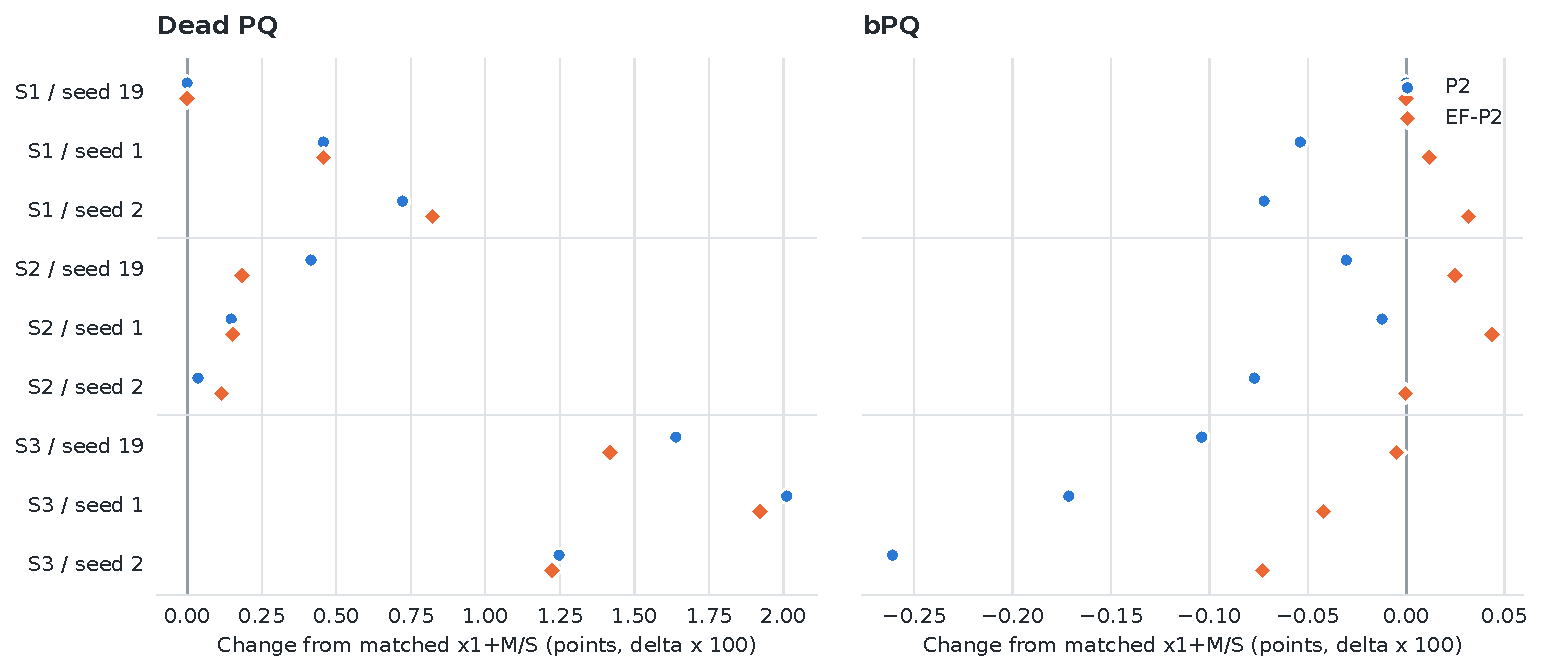
\includegraphics[width=\linewidth]{figs/paired_gains_en.pdf}
\caption{Each split--seed pair relative to its own x1+M/S baseline. Circles denote P2 and diamonds EF-P2. Changes are plotted on a 100-point scale (raw $\Delta\times100$). Both methods have eight positive Dead differences and one unchanged pair; EF-P2 bPQ results are closer to zero. A zero difference is not counted as an improvement.}
\label{fig:pairs}
\end{figure}

Under the pre-registered rule, EF-P2's mean Dead gain of 0.00699 exceeds the maximum paired-difference standard deviation of 0.00337, with eight positive pairs and one zero. The mean paired mPQ difference is positive, and the mean paired bPQ difference is above its lower bound of $-0.000279$. EF-P2 therefore \textbf{passes the rule} and replaces P2 as the reporting candidate. Passing is strictly limited to that rule.

\subsection{Uncertainty and split dependence remain}

Each split receives 2,000 tissue-stratified paired-image bootstrap replicates, with random seed 20261004. The three trained seeds share the same resampled image indices, after which their paired differences are averaged. Splits are not pooled. Table~\ref{tab:ci} and Figure~\ref{fig:ci} show the EF-P2 results.

\begin{table}[H]
\centering\small
\caption{EF-P2 minus the same-seed baseline: three-seed mean differences within each split and 95\% paired-image bootstrap intervals.}
\label{tab:ci}
\begin{tabular}{llrr}\toprule
Split & Metric & Mean difference & 95\% interval\\\midrule
split 1 & mPQ & +.000653 & [$-$.000324, +.001566]\\
 & bPQ & +.000145 & [$-$.000709, +.000944]\\
 & Dead PQ & +.004265 & [+.000962, +.007959]\\\midrule
split 2 & mPQ & +.000445 & [$-$.000317, +.001197]\\
 & bPQ & +.000228 & [$-$.000492, +.000880]\\
 & Dead PQ & +.001505 & [$-$.000534, +.003594]\\\midrule
split 3 & mPQ & +.000944 & [$-$.000462, +.002469]\\
 & bPQ & $-$.000400 & [$-$.001567, +.000781]\\
 & Dead PQ & +.015204 & [+.005719, +.026246]\\\bottomrule
\end{tabular}
\end{table}

\begin{figure}[H]
\centering
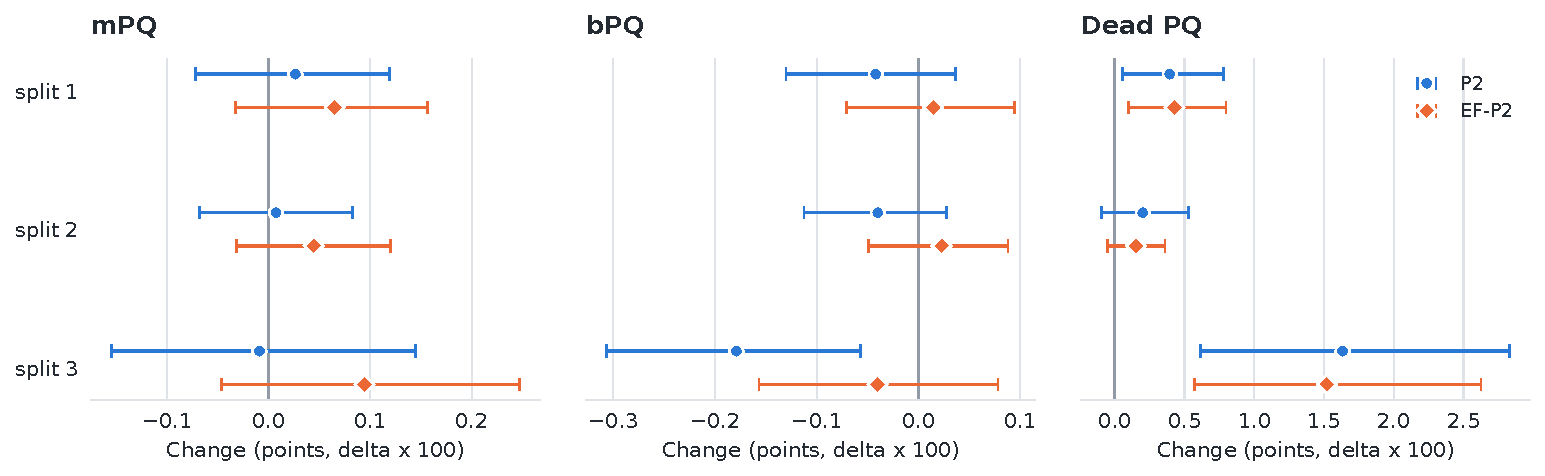
\includegraphics[width=\linewidth]{figs/split_intervals_en.pdf}
\caption{Per-split intervals for P2 and EF-P2. Each panel has its own horizontal scale, expressed as 100-point score differences. After filtering, the split-3 bPQ interval changes from entirely below zero to spanning zero; this does not prove the absence of bPQ loss. The largest Dead improvement remains in split 3.}
\label{fig:ci}
\end{figure}

Dead intervals exclude zero in splits 1 and 3 but span zero in split 2. All mPQ and bPQ intervals span zero. These intervals are \textbf{conditional on the three already trained seeds}; they do not include all uncertainty from training new models. With only three seeds per split, the standard-deviation estimates themselves are also unstable.

The stricter metrics retain a warning: mean strict mPQ is 0.00030 lower under EF-P2, and split-2 mean strict Dead PQ is approximately 0.00013 lower. Improvements in the overall average and official Dead metric do not remove costs for every class or every split.

\section{Additional evidence from the border audit}

After EF execution, an error was found in the existence audit's border grouping. The old table incorrectly used an area bin and returned zero for both border and interior rows. Table~\ref{tab:border} was regenerated from the frozen validation predictions after correction. Other grouped tables and legacy columns in the candidate records remain unchanged. The EF menu did not depend on the old border table, so the nine EF scores are unaffected.

\begin{table}[H]
\centering\small
\caption{Post-execution reconstruction of border groups for validation additions only. Border means contact with any edge of the native prediction map. This table was not used to design the EF menu.}
\label{tab:border}
\begin{tabular}{lrrrr}\toprule
Location & Additions & Matches & Match rate & \shortstack{Matched and\\correctly typed Dead}\\\midrule
Border-touching & 9,975 & 5,273 & 52.86\% & 85\\
Interior & 7,384 & 1,931 & 26.15\% & 614\\\bottomrule
\end{tabular}
\end{table}

These results do not support discarding candidates solely because they touch the border. The border group has a higher overall matching rate, while most correctly recovered Dead nuclei are interior. The groups differ in class, area, and fold composition, so the difference is not a causal effect of location or a reason to immediately add another filter. The frozen menu remains unchanged.

A fallback branch in the EF test entry point was also corrected that day. If stage-one P2 is non-identity but stage-two EF selects identity, all additions must be cancelled. The only EF identity pair among the archived nine already had stage-one identity and did not exercise the bug; a regression test now covers the missing combination. Source fingerprints in old selection manifests were not rewritten. Provenance checks should not be bypassed to present old and new code as the same execution.

\section{Current progress and next steps}

\subsection{Completed work}

Baseline reproduction, unified evaluation, tests of the first three research directions, and the two historical reports are complete. This stage additionally completes the P0--P3 audit, typing-confidence audit, nine-pair matched-seed validation, validation-only existence audit, and pre-registered EF-P2 experiment. Code review found no new confirmed defect sufficient to overturn these results. The full test suite run on October 6, including a new report-font regression test, returned \textbf{157 passed, 63 warnings}; most warnings concern dependency deprecations. This establishes that the current regression tests pass, not that all possible implementation errors have been excluded.

The research log\cite{findings} is used to trace the experimental history, not as the final numerical source. Raw evaluation summaries were used to extract six endpoint differences for each of nine pairs in each of two rounds, giving 108 differences checked against the statistics files. Area and corrected border groups were then recomputed from candidate records. Extraction, independent verification, and plotting code are kept in \code{scripts/} for reproducibility.

\subsection{Conclusions that remain unsupported}

\begin{enumerate}
\item \textbf{Universal superiority.} Most of the gain is in Dead. Overall mPQ improves only slightly, and strict mPQ declines slightly.
\item \textbf{Independent confirmation.} EF is the third pre-registered test read in the sequence P0--P3 v2, matched-seed, and EF. Earlier mechanism studies also examined these images. Validation-only parameter selection within each round does not eliminate adaptation to prior test findings across rounds.
\item \textbf{A cost-free improvement.} Area filtering itself uses only CPU computation, but its candidates require both x1 and x2 predictions. Complete inference latency, peak resource use, and energy have not been measured.
\item \textbf{Independent checkpoint binding for every historical prediction.} Old NPZ files do not contain checkpoint hashes. Some provenance relies on saved configurations and sidecar manifests. Input hashes protect a frozen snapshot but cannot retrospectively create missing checkpoint bindings.
\item \textbf{Generalization beyond the present setting.} EF-P2 has not been confirmed on independent external data, a patient-level resplit, or additional seeds. The results do not establish validity for pathology applications.
\end{enumerate}

\subsection{Prioritize confirmation rather than a larger menu}

EF-P2 should now remain frozen, without adding shape thresholds, class thresholds, or consistency rules using these test images. The most useful next experiment is a comparison of x1+M/S, P2, and EF-P2 on pre-specified independent data or a new strict holdout design, with Dead gains, acceptable overall losses, and cost endpoints registered in advance. If independent data are unavailable, the present findings should remain explicitly exploratory rather than treating further reuse of the same source data as confirmation.

A second priority is to measure the entire pipeline, including both sets of predictions and final post-processing, rather than timing the area filter alone. A third is a qualitative audit with a pre-fixed sampling rule: show recovered Dead nuclei, removed false positives, wrongly removed true positives, and failures across splits. Examples should explain the mechanism, not drive threshold reselection.

The defensible conclusion is that \textbf{separating type confidence from instance reliability can retain most of the Dead benefit supplied by scale complementarity while reducing the average loss in overall segmentation}. Whether this repeats on new data, and whether the benefit warrants an additional higher-scale model, remain questions for the next stage.

\appendix
\section{Files, numerical sources, and reproduction entry points}

Portable report files are collected in \code{docs/report/stage_report_3/}. The formal Chinese and English editions and the plain-language Chinese digest are supplied as TeX and PDF. The \code{figs/} directory contains figures and their numerical CSV counterparts; \code{verified_numbers.json} stores a verification snapshot of the main table and existence statistics. Model weights, raw data, machine configuration, and credentials are not included.

\begin{table}[H]
\centering\footnotesize
\caption{Main experiment-artifact roots, relative to \code{runs/analysis/}. These are local outputs and are not distributed through Git.}
\begin{tabularx}{\linewidth}{lY}\toprule
Directory & Use in this report\\\midrule
\code{p0p3_20261002_v2/} & Seed-19 scale controls, P1 diagnostics, initial P2, and the P3 validation probe.\\
\code{typing_audit_20261003/} & Matching rates, typing accuracy conditional on matching, and confidence transfer.\\
\code{matched_seed_20261004/} & Nine-pair P0/P2 selections, test evaluations, differences, and bootstrap statistics.\\
\code{existence_ef_20261005/} & Nine-pair EF selections, test evaluations, and statistics under the same conventions.\\
\code{existence_audit_20261005_v2/} & Rechecked candidate records, area groups, and border groups.\\\bottomrule
\end{tabularx}
\end{table}

Use the pinned dependency environment and run the following extraction or plotting commands from the repository root:
\begin{quote}\small
\code{python scripts/report3_numbers.py}\\
\code{python scripts/verify_report3.py}\\
\code{python scripts/make_report_figures3.py}\\
\code{python -m pytest -q}
\end{quote}
The verification script fails when required artifacts are missing or numbers disagree; it does not modify experiment outputs. The old existence-audit path used by \code{report3_numbers.py} contributes only unchanged non-border groups. Border values in this report come exclusively from v2. Re-executing historical selection and evaluation also requires a matching source snapshot; frozen manifests must not be edited simply to pass provenance checks.

\begin{thebibliography}{9}
\bibitem{pannuke} J. Gamper, N. Alemi Koohbanani, K. Benes, et al. PanNuke Dataset Extension, Insights and Baselines. arXiv:2003.10778, 2020. \url{https://arxiv.org/abs/2003.10778}.
\bibitem{reports} bdd26 project. Stage Reports I and II, with October 2, 2026 correction addenda. \code{docs/report/stage_report_1/} and \code{docs/report/stage_report_2/}.
\bibitem{p0p3} bdd26 project. P0--P3 execution results and research assessment, v2, October 2, 2026. \code{docs/P0_P3_RESULTS_2026-10-02.md}.
\bibitem{uni} R. J. Chen, T. Ding, M. Y. Lu, et al. Towards a general-purpose foundation model for computational pathology. \emph{Nature Medicine}, 30(3):850--862, 2024. \url{https://doi.org/10.1038/s41591-024-02857-3}.
\bibitem{cellvit} F. H\"orst, M. Rempe, L. Heine, et al. CellViT: Vision Transformers for precise cell segmentation and classification. \emph{Medical Image Analysis}, 94:103143, 2024. \url{https://doi.org/10.1016/j.media.2024.103143}.
\bibitem{pq} A. Kirillov, K. He, R. Girshick, et al. Panoptic Segmentation. In \emph{CVPR}, pp. 9396--9405, 2019. \url{https://doi.org/10.1109/CVPR.2019.00963}.
\bibitem{matchedplan} bdd26 project. Pre-registered matched-seed validation protocol, October 3, 2026, with execution annotations. \code{docs/superpowers/plans/2026-10-03-matched-seed-validation.md}.
\bibitem{efplan} bdd26 project. Existence-filtered P2 pre-registered protocol, October 5, 2026, with post-execution audit notes. \code{docs/superpowers/plans/2026-10-05-existence-filter-p2.md}.
\bibitem{findings} bdd26 project. Experiment log, entries for October 3--5, 2026. \code{docs/findings.md}.
\end{thebibliography}
\end{document}
